% Drawing 43/09-1 -- folder 43, batch 09, archive page 177 (PDF page 178).
% Transcription: en haut, deux figures d'ovales qui se chevauchent, séparées par un trait vertical ; les noms des classes sont écrits sur les ovales et les groupes dans les régions, séparés par des traits obliques. À gauche : « $k$-connexe », « multiplicatif », « fini séparable », « unipotent », avec $(\mathbb{G}_m)$, $(\mu_p)$, $(\mathbb{Z}/\ell\mathbb{Z})$, $(\mathbb{G}_a, \alpha_p)$, $(\mathbb{Z}/p\mathbb{Z})$. À droite : « infinitésimal », « discret sép. », « sans torsion additive », « sans torsion multiplicative », avec $(\alpha_p, \mathbb{V})$, $(\mu_p)$, $(\mathbb{Z}/\ell\mathbb{Z})$, $(\mathbb{Z}/p\mathbb{Z})$, $(\mathbb{Z})$, $(\mu_p, \mathbb{V})$.
% Kind: two diagrams of overlapping ovals (classes of group schemes) with groups in the regions. Method 2 (redraw from the facsimile). Status: partial.
% Notes: Redrawn from the colour scan at 400 dpi, every coordinate read on gridded crops and the result overlaid on the page. The ovals are open arcs on the page and are drawn as the arcs they are, each through points read on it: on the left seven arcs (the wide arc under « k-connexe », an inner arc under the second writing of « multiplicatif », two arcs below (G_m) and (Z/lZ), the oval of « fini séparable » in two arcs, and an inner arc beside « unipotent k-connexe »); on the right five arcs (the left oval in two arcs, the arc under « discret sép. », the long arc running from the left oval to the right, and a stroke under it). The oblique strokes that separate the groups are drawn where they are (eight on the left, two of them crossed by a tick; four on the right), with the heavy dot from which one of them starts, the heavy underlines of (G_m) and (Z), and the underlines of the class names. The vertical double stroke separates the two figures. All unstruck writing was read again on the scan. Left: « k-connexe », « multiplicatif k-connexe » (second, smaller writing, uncertain), « multiplicatif séparable » (smaller), « multiplicatif », « fini séparable », « unipotent », « unipotent k-connexe » (smaller); groups (G_m), (mu_p) twice, (G_a, alpha_p) twice, (Z/lZ) three times, Z/pZ twice. Right: « discret sép. », « sans torsion additive », « sans torsion multiplicative »; groups (alpha_p, V), (mu_p) twice, Z/lZ twice, (Z/pZ), (Z), (mu_p, V). Left out, as struck on the page: at the left the word « Unipotent » under (G_a, alpha_p), a blackened group below (mu_p) and a struck word in the upper right oval; at the right the words « infinitésimal » (twice), « discret », « (séparable) », and three groups, Z/pZ and (Z/lZ) at the top and a Z/lZ under a cross at the centre. Still differs: whether an oblique stroke that runs over a group separates it from its neighbour or strikes it is a reading (taken as separating for (Z/lZ) and (Z/pZ) in the upper right oval of the left figure and for the lower (mu_p) of the right figure); the arcs do not close, so the picture does not by itself fix the incidence of classes and groups; the writing is set in print at about its place. Redrawn 2026-11-12 (issue 128): to check again. 2026-11-13, Claude Opus 5.5, overlay check: redrawn from the 228 ppi scan (its own resolution) on millimetre grids, since the previous coordinates lay 1 to 3 units off the ink; compiled with tectonic and laid over the crop; the arcs and strokes lie on the ink to within about 1 unit. Changed: every arc re-read (the lower arc of the fini séparable oval now runs on round its right side to (54.7,14.2); the outer lower arc of the left figure ends at the top of the blackened group); in the right figure the lower arc of the left oval runs up into a hatched struck scribble after (mu_p, V), and two strokes leave to the right, one from the dot and one from the hatching, joining near the hooked end (the old « stroke under it » was misplaced); the struck words are drawn in the struck style as Michel's rule asks (#146): « Unipotent » under (G_a, alpha_p), Z/pZ and (Z/lZ) at the top right, the crossed Z/lZ at the centre, « discret » and « (séparable) », and the lower « infinitésimal ». Re-read: the upper « infinitésimal » of the right figure is not struck, it sits on the top of the left oval, which underlines it, so it is drawn as a class name (as the transcription has it); « sans torsion additive » is written in two lines under the struck lower « infinitésimal », « sans torsion multiplicative » in two lines at the right. Class names set \scriptsize (\tiny for « unipotent k-connexe ») so that they do not cover the groups; groups at \small. Still differs: the struck word under the heavy stroke in the upper right oval of the left figure and the blackened group below (mu_p) are not readable and are drawn as their strike strokes only; the hatched scribble after (mu_p, V) is not readable either; whether an oblique stroke over a group separates or strikes it remains a reading; the print is larger than the hand.
% Coordinates: 1 unit = 1 mm = 1/100 of the crop width, y downwards as on the crop (bbox in page fractions: [0.07, 0.055, 0.97, 0.32]).
% Redrawn by Claude (claude-fable-5-2), issue #128, 2026-11-12, from the colour scan at 350 dpi; not checked by a human; not compiled (no TeX in the session).
% Rights: reproduces part of the work -- behind RENDER_TRANSCRIPTS, never published by itself.
\documentclass[tikz,border=3pt]{standalone}
\usepackage{amsmath,amssymb}
\usetikzlibrary{patterns,arrows.meta}
\tikzset{pencil/.style={black!45}, struck/.style={black!35}, mpt/.style={circle,draw,inner sep=1.3pt}, pt/.style={circle,fill,inner sep=0.9pt}, opt/.style={circle,draw,fill=white,inner sep=1.1pt}, Rd/.style={red!75!black}, Gn/.style={green!45!black}, Br/.style={brown!70!black}, Bl/.style={blue!70!black}}
\begin{document}
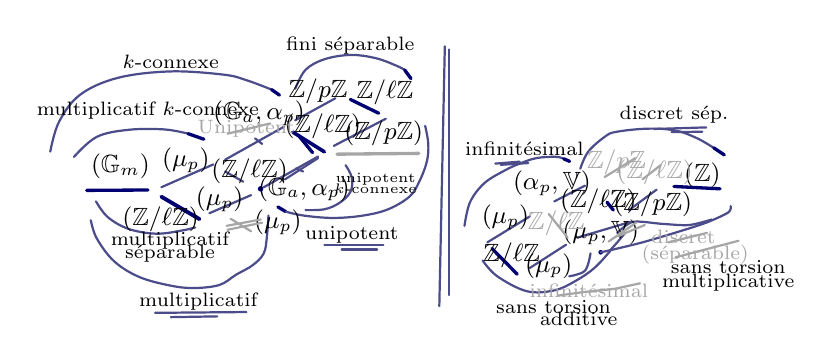
\begin{tikzpicture}[x=1mm,y=-1mm,line cap=round,line join=round,font=\small]
\tikzset{ink/.style={thick,blue!35!black!70}, heavy/.style={very thick,blue!45!black}, sk/.style={struck,thick}}
% ---------------- left figure ----------------
% the wide arc under « k-connexe »
\draw[ink] plot[smooth, tension=0.6] coordinates {(7.09,17.48) (8.2,13.7) (10.9,10.24) (15.7,8.1) (22.4,7.29) (29.1,7.7) (32.0,8.4) (35.2,9.6)};
\draw[heavy] (35.2,9.6) -- (36.2,10.3);
% the inner arc under « multiplicatif k-connexe »
\draw[ink] plot[smooth, tension=0.6] coordinates {(10.1,18.15) (13.0,15.6) (17.1,14.7) (21.6,14.66) (24.6,15.2)};
\draw[heavy] (24.6,15.2) -- (26.6,15.9);
% the arc round (Z/lZ) and the outer arc under it
\draw[ink] plot[smooth, tension=0.6] coordinates {(12.9,23.8) (14.4,25.8) (17.06,27.3) (20.55,27.9) (23.8,27.5) (25.5,27.1)};
\draw[ink] plot[smooth, tension=0.6] coordinates {(12.24,26.2) (13.0,28.5) (15.2,31.4) (18.4,33.4) (22.4,34.5) (25.4,34.8) (28.6,34.4) (30.7,33.1) (32.8,31.9) (34.2,30.4) (34.6,28.3) (34.8,25.6)};
% the oval of « fini séparable »: upper arc, and the lower arc running round to the right
\draw[ink] plot[smooth, tension=0.6] coordinates {(38.2,9.5) (39.5,7.1) (41.9,5.75) (45.2,5.2) (48.4,5.6) (51.05,6.56) (52.1,7.1)};
\draw[heavy] (52.1,7.1) -- (52.9,8.2);
\draw[heavy] (36.0,24.5) -- (37.0,25.1);
\draw[ink] plot[smooth, tension=0.6] coordinates {(37.0,25.1) (39.3,25.6) (43.0,25.9) (46.8,25.6) (50.0,24.8) (52.7,23.2) (53.9,21.4) (54.9,18.8) (55.1,16.5) (54.7,14.2)};
% the inner arc beside « unipotent k-connexe »
\draw[ink] plot[smooth, tension=0.6] coordinates {(44.6,19.2) (45.4,20.8) (45.2,22.6) (43.8,24.0) (41.9,24.8) (39.5,24.9)};
% separating strokes
\draw[heavy] (11.7,22.4) -- (19.5,22.35);
\draw[ink] (21.2,22.0) -- (27.8,19.1);
\draw[heavy,line width=1.4pt] (21.2,23.2) -- (26.05,26.05);
\draw[ink] (29.3,18.5) -- (36.8,14.3);
\draw[ink] (33.1,15.8) -- (34.0,16.5);
\draw[ink] (29.3,20.0) -- (31.6,21.3);
\draw[ink] (27.3,25.3) -- (32.6,23.0);
\draw[ink] (34.2,22.0) -- (41.1,18.1);
\draw[ink] (36.9,21.0) -- (41.1,18.3);
\draw[ink] (38.3,19.6) -- (39.2,20.0);
\fill[blue!45!black] (33.8,22.2) circle[radius=0.35];
\draw[ink] (38.2,13.5) -- (43.3,10.7);
\draw[heavy] (45.2,10.85) -- (48.8,12.6);
\draw[heavy,line width=1.3pt] (37.9,15.0) -- (41.9,17.5);
\draw[heavy] (38.6,15.4) -- (40.4,17.6);
\draw[ink] (43.1,16.75) -- (49.7,13.3);
% writing (class names, then groups)
\node at (22.4,6.1) {\scriptsize $k$-connexe};
\node at (19.5,12.25) {\scriptsize multiplicatif $k$-connexe};
\node[align=center,font=\scriptsize] at (22.3,29.6) {multiplicatif\\[-3pt]s\'eparable};
\node at (25.9,36.5) {\scriptsize multiplicatif};
\draw[ink] (20.4,37.95) -- (32.0,37.85);
\draw[ink] (22.4,38.5) -- (28.3,38.4);
\node at (45.2,4.0) {\scriptsize fini s\'eparable};
\node at (45.4,28.1) {\scriptsize unipotent};
\draw[ink] (41.9,29.3) -- (49.4,29.3);
\draw[ink] (44.1,29.9) -- (48.6,29.9);
\node[align=center,font=\tiny] at (48.4,21.5) {unipotent\\[-2pt]$k$-connexe};
\node at (16.0,19.35) {$(\mathbb{G}_m)$};
\node at (24.3,18.55) {$(\mu_p)$};
\node at (21.1,26.05) {$(\mathbb{Z}/\ell\mathbb{Z})$};
\node at (33.6,12.6) {$(\mathbb{G}_a,\alpha_p)$};
\node at (32.4,20.0) {$(\mathbb{Z}/\ell\mathbb{Z})$};
\node at (28.6,23.5) {$(\mu_p)$};
\node at (39.3,22.2) {$(\mathbb{G}_a,\alpha_p)$};
\node at (41.1,9.8) {$\mathbb{Z}/p\mathbb{Z}$};
\node at (49.6,10.0) {$\mathbb{Z}/\ell\mathbb{Z}$};
\node at (41.7,14.2) {$(\mathbb{Z}/\ell\mathbb{Z})$};
\node at (49.45,15.1) {$(\mathbb{Z}/p\mathbb{Z})$};
\node at (36.0,26.5) {$(\mu_p)$};
% struck on the page
\node[struck] at (32.0,14.6) {\scriptsize Unipotent};
\draw[sk] (29.6,15.2) -- (35.0,13.9);
\draw[sk] (29.5,26.9) -- (33.8,26.1);  \draw[sk] (29.6,27.4) -- (34.0,26.5);  \draw[sk] (30.0,26.0) -- (32.6,27.6);
\draw[heavy,struck] (43.5,17.8) -- (53.9,17.7);
% ---------------- vertical double stroke ----------------
\draw[ink] (57.2,4.1) -- (56.5,37.1);
\draw[ink] (57.7,4.5) -- (57.7,35.7);
% ---------------- right figure ----------------
% the left oval: upper arc (its top underlines « infinitésimal »), lower arc, closing piece
\draw[ink] plot[smooth, tension=0.6] coordinates {(59.7,26.9) (60.4,23.9) (62.2,21.5) (64.75,19.9) (66.7,19.0) (68.88,18.29) (71.33,18.14) (72.3,18.39)};
\draw[heavy] (72.3,18.39) -- (73.05,18.71);
\draw[ink] (63.6,19.0) -- (66.7,18.75);
\draw[ink] (64.3,19.15) -- (67.8,18.93);
\draw[ink] plot[smooth, tension=0.6] coordinates {(62.0,31.3) (63.85,33.3) (67.6,35.2) (71.1,35.1) (73.8,33.9) (76.2,32.25) (78.2,30.1)};
\draw[ink] plot[smooth, tension=0.6] coordinates {(73.0,33.3) (75.0,32.6) (75.7,30.4)};
% the upper right oval
\draw[ink] plot[smooth, tension=0.6] coordinates {(74.4,19.65) (75.4,17.5) (77.5,15.6) (79.0,14.96) (83.0,14.56) (86.5,14.8) (89.2,15.76) (91.35,17.0)};
\draw[heavy] (91.35,17.0) -- (92.7,17.9);
% the two long strokes to the right: from the dot, and from the hatching
\fill[blue!45!black] (77.0,30.26) circle[radius=0.3];
\draw[ink] plot[smooth, tension=0.5] coordinates {(77.0,30.26) (78.2,30.0) (82.3,29.0) (86.7,27.7) (90.4,26.5) (93.2,25.2) (93.5,24.4)};
\draw[ink] plot[smooth, tension=0.5] coordinates {(78.2,30.0) (79.1,29.0) (80.1,27.8)};
\draw[ink] plot[smooth, tension=0.5] coordinates {(79.1,27.8) (81.1,26.4) (84.8,26.65) (88.2,26.8) (91.1,26.1)};
% separating strokes
\draw[ink] (71.1,23.8) -- (75.0,21.8);
\draw[ink] (62.6,29.0) -- (68.0,25.7);
\draw[heavy] (63.2,29.8) -- (66.4,33.05);
\draw[ink] (68.0,32.25) -- (72.6,29.3);
\draw[ink] (74.0,28.4) -- (80.8,26.4);
\draw[heavy] (77.8,23.9) -- (78.6,24.9);
\draw[ink] (80.6,24.9) -- (84.1,22.3);
\draw[heavy] (86.3,21.9) -- (92.15,22.2);
\draw[ink] (83.8,14.6) -- (90.4,14.4);
\draw[ink] (86.0,15.0) -- (89.9,14.95);
% writing
\node at (67.3,17.1) {\scriptsize infinit\'esimal};
\node at (86.3,12.8) {\scriptsize discret s\'ep.};
\node at (71.0,37.2) {\scriptsize sans torsion};
\node at (74.2,38.7) {\scriptsize additive};
\node[align=center,font=\scriptsize] at (93.2,33.3) {sans torsion\\[-3pt]multiplicative};
\node at (70.8,21.5) {$(\alpha_p,\mathbb{V})$};
\node at (64.9,25.8) {$(\mu_p)$};
\node at (65.7,30.6) {$\mathbb{Z}/\ell\mathbb{Z}$};
\node at (70.4,32.0) {$(\mu_p)$};
\node at (76.7,23.8) {$(\mathbb{Z}/\ell\mathbb{Z})$};
\node at (77.0,27.7) {$(\mu_p,\mathbb{V})$};
\node at (83.6,24.2) {$(\mathbb{Z}/p\mathbb{Z})$};
\node at (89.9,20.45) {$(\mathbb{Z})$};
% struck on the page
\node[struck] at (71.35,26.6) {$\mathbb{Z}/\ell\mathbb{Z}$};
\draw[sk] (70.4,25.4) -- (72.8,28.4);
\node[struck] at (79.0,18.85) {$\mathbb{Z}/p\mathbb{Z}$};
\draw[sk] (77.5,20.7) -- (81.4,18.3);
\node[struck] at (83.85,20.05) {$(\mathbb{Z}/\ell\mathbb{Z})$};
\draw[sk] (82.3,21.0) -- (84.6,19.2);
\draw[sk] (78.0,28.9) -- (81.5,26.5);  \draw[sk] (79.2,28.2) -- (82.6,26.8);
\node[struck] at (75.5,35.2) {\scriptsize infinit\'esimal};
\draw[sk] (71.65,35.75) -- (74.9,35.3) -- (78.8,34.9) -- (82.0,34.2);
\node[struck] at (87.5,28.3) {\scriptsize discret};
\draw[sk] (85.6,29.0) -- (90.5,27.8);
\node[struck] at (89.0,30.6) {\scriptsize (s\'eparable)};
\draw[sk] (86.5,30.9) -- (94.5,28.8);
\end{tikzpicture}
\end{document}
